\documentclass{article}
\usepackage{amsmath}
\usepackage{graphicx}  % Paquete para incluir imágenes
\usepackage{float}
\usepackage{amsmath,amssymb,  graphicx, float}
\usepackage{geometry}
\usepackage[table]{xcolor}
\geometry{top=2cm, bottom=2cm, left=2.5cm, right=2.5cm}

\begin{document}
Alberto Arath Figueroa Salomon 
\newpage
\begin{flushleft}
Se tiene una neurona con los siguientes pesos $w_0=-4$, $w_1=3$, $w_2=1$ y función de activación
Hacer lo siguiente:

\begin{enumerate}
\item Dibuje la neurona con sus pesos y sus entradas y salida mostrando la entrada que está fija a 1.
\item Calcular el producto $W^T X$ y graficarlo en GeoGebra 3D.
\[ wtx(x_1, x_2) = 3 x_1 + x_2 - 4 \]
\begin{figure}[H]
  \centering
  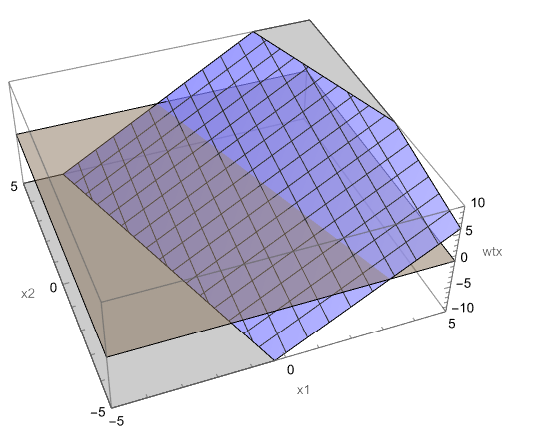
\includegraphics[width=0.5\textwidth]{Imagen0.png}  % Cambia el nombre del archivo y su ruta según sea necesario
\end{figure}
\item Encontrar la ecuación de la recta que divide al espacio de entrada en 2 partes y graficarla usando GeoGebra 2D.
\[ 0 = 3 x_1 + x_2 - 4 \]
\begin{figure}[H]
  \centering
  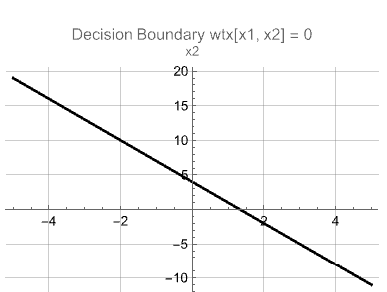
\includegraphics[width=0.5\textwidth]{Imagen1.png}  % Cambia el nombre del archivo y su ruta según sea necesario
\end{figure}
\newpage
\item Graficar en GeoGebra 3D la salida de la neurona $y$.
\begin{figure}[H]
  \centering
  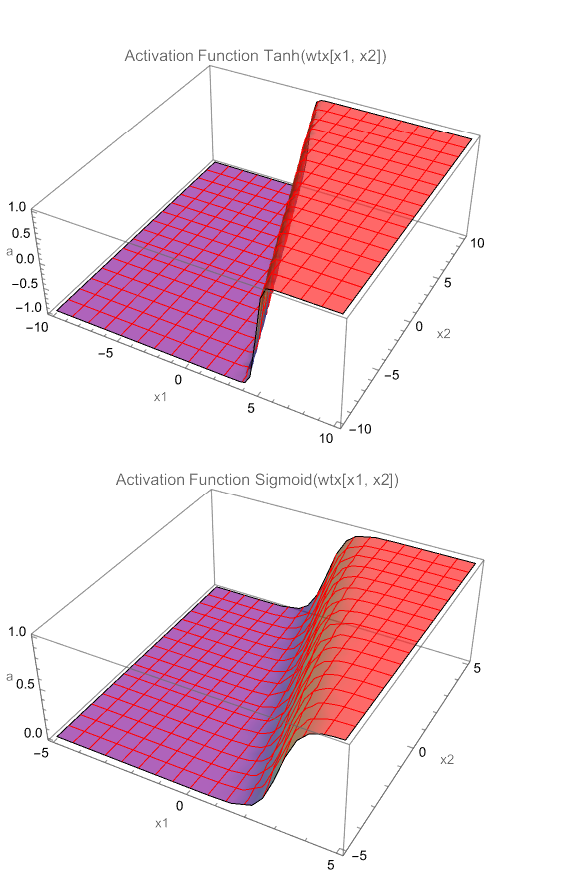
\includegraphics[width=0.5\textwidth]{1d.png}  % Cambia el nombre del archivo y su ruta según sea necesario
\end{figure}
\end{enumerate}
Diseñar una neurona que divida el espacio de entrada $(x_1, x_2)$ con una línea recta con pendiente
$m=3$, $b=-2$ (b es el valor que toma el eje $x_2$ cuando $x_1=0$, es decir, donde la recta cruza con el eje
$x_2$) y función de activación $f(wtx)=\text{Sigmoide}$. Una vez diseñada la neurona haga lo siguiente:
\begin{enumerate}
  \item Dibuje la neurona con sus pesos y sus entradas y salida mostrando la entrada que está fija a 1.
  \item Calcular el producto $W^T X$ y graficarlo en GeoGebra 3D.
  \[ wtx(x_1, x_2) = -3 x_1 + x_2 + 2 \]
  \begin{figure}[H]
    \centering
    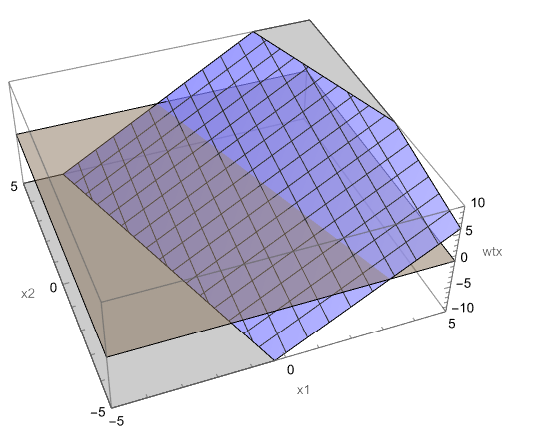
\includegraphics[width=0.5\textwidth]{Imagen0.png}  % Cambia el nombre del archivo y su ruta según sea necesario
  \end{figure}
  \item Encontrar la ecuación de la recta que divide al espacio de entrada en 2 partes y graficarla usando GeoGebra 2D.
  \[ 0 = -3 x_1 + x_2 + 2 \]
  \begin{figure}[H]
    \centering
    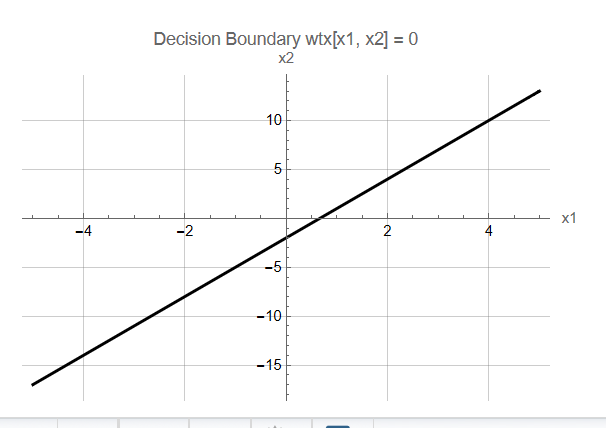
\includegraphics[width=0.5\textwidth]{2_Decision_boundry.PNG}  % Cambia el nombre del archivo y su ruta según sea necesario
  \end{figure}
  \newpage
  \item Graficar en GeoGebra 3D la salida de la neurona $y$.
  \begin{figure}[H]
    \centering
    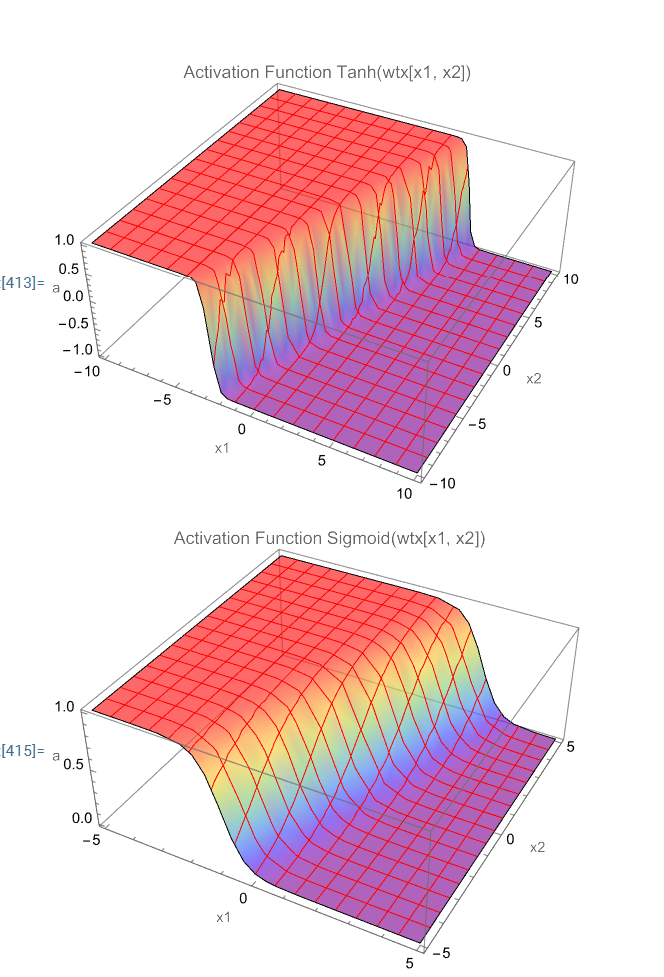
\includegraphics[width=0.5\textwidth]{2_output_neuron.PNG}  % Cambia el nombre del archivo y su ruta según sea necesario
  \end{figure}
  \end{enumerate}

  3. Diseñe una neurona que tenga a la recta $x_2=-x_1+2$ como la recta que divide el espacio de entrada $(x_1,x_2)$ con 
  función de activación $f(wtx)=\text{Lineal}$. Una vez diseñada la neurona haga lo siguiente:
  \begin{enumerate}
    \item Dibuje la neurona con sus pesos y sus entradas y salida mostrando la entrada que está fija a 1.
    \item Calcular el producto $W^T X$ y graficarlo en GeoGebra 3D.
    \[ wtx(x_1, x_2) = - x_1 - x_2 + 2 \]
    \begin{figure}[H]
      \centering
      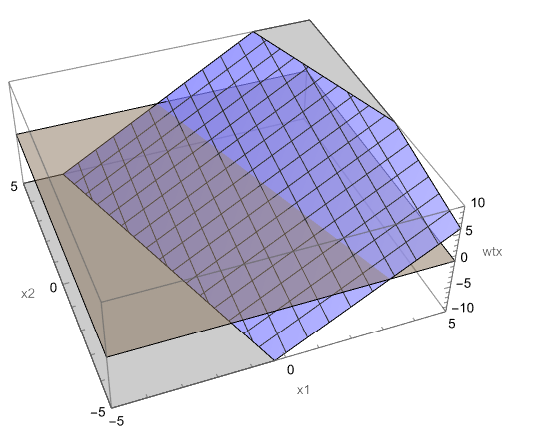
\includegraphics[width=0.5\textwidth]{Imagen0.png}  % Cambia el nombre del archivo y su ruta según sea necesario
    \end{figure}
    \item Encontrar la ecuación de la recta que divide al espacio de entrada en 2 partes y graficarla usando GeoGebra 2D.
    \[ 0 = - x_1 - x_2 + 2 \]
    \begin{figure}[H]
      \centering
      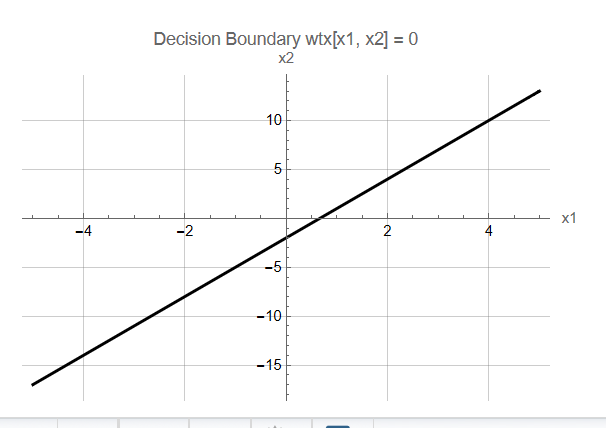
\includegraphics[width=0.5\textwidth]{2_Decision_boundry.PNG}  % Cambia el nombre del archivo y su ruta según sea necesario
    \end{figure}
    \item Graficar en GeoGebra 3D la salida de la neurona $y$.
    \begin{figure}[H]
      \centering
      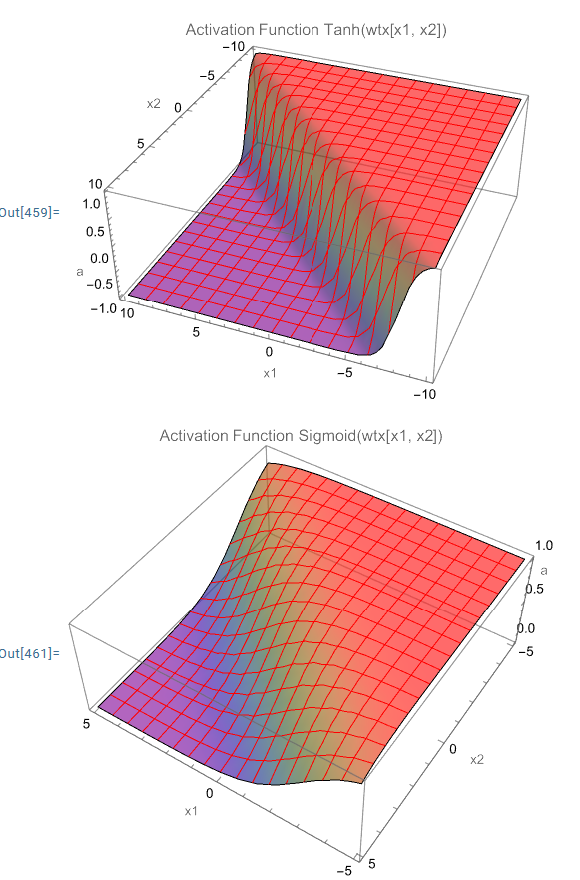
\includegraphics[width=0.5\textwidth]{3_d.PNG}  % Cambia el nombre del archivo y su ruta según sea necesario
    \end{figure}
    \end{enumerate}

\newpage
4. Considerando la siguiente red neuronal:
\begin{enumerate}
  \item
   Encontrar la ecuación de la recta cuando Wtx = 0 para cada neurona
   \[ 0 =   2x_1   - 2x_2  + 1 \]
   \[ 0 =   2x_1 - 2x_2 - 1 \]
   \[ 0 =   2x_1 - 2x_2 - 1 \]
  \item Graficar la ecuación de la recta para cada una de las neuronas en el ejercicio 1 

  \begin{figure}[H]
    \centering
    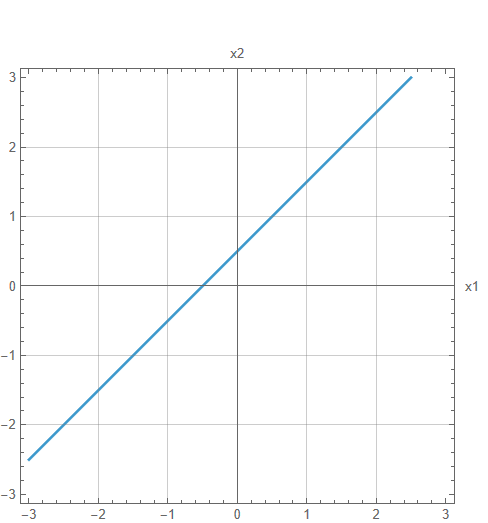
\includegraphics[width=0.5\textwidth]{4_a_1.PNG}  
  \end{figure}
  \begin{figure}[H]
    \centering
    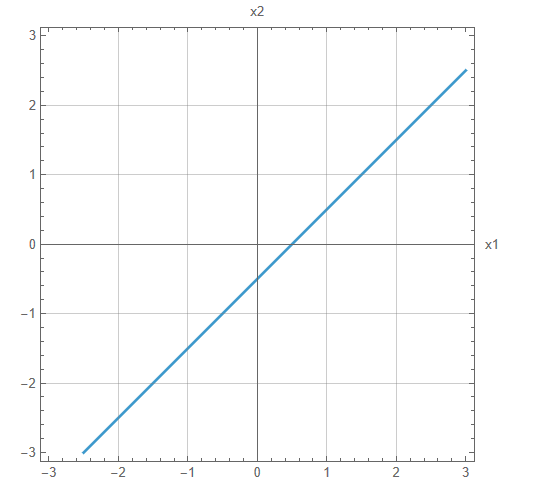
\includegraphics[width=0.5\textwidth]{4.a.2.PNG}
  \end{figure}
  \begin{figure}[H]
    \centering
    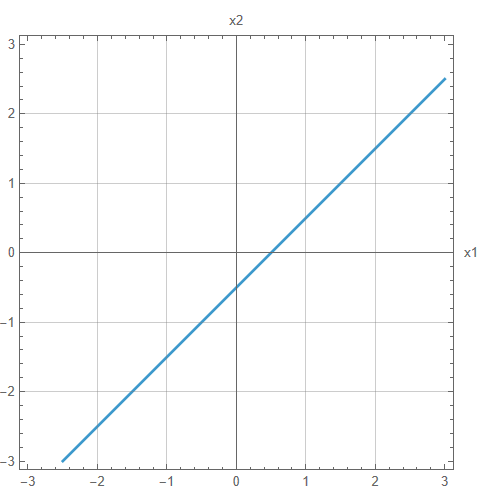
\includegraphics[width=0.5\textwidth]{4_a_3.PNG} 
  \end{figure}

  \item Encontrar la función de salida para cada neurona
  \begin{enumerate}
    \item \(\frac{1}{e^{-2x_1 + 2x_2 - 1} + 1}\)
  

    \item \(\frac{1}{e^{-2x_1 + 2x_2 + 1} + 1}\)
    

    \item \(\frac{1}{e^{-2x_1 + 2x_2 + 1} + 1}\)

  \end{enumerate}

  \item Obtener la funcion de salida y(x1, x2) con respecto a alas demas entradas x1, x2 de la red neuronal completa$y$.
  \[
  -\frac{2}{e^{-2x_1+2x_2-1}+1} + \frac{2}{e^{-2x_1+2x_2+1}+1} - 1
  \]
 
  \item Graficar las funciones obtenidas en 3 y 4
  \begin{figure}[H]
    \centering
    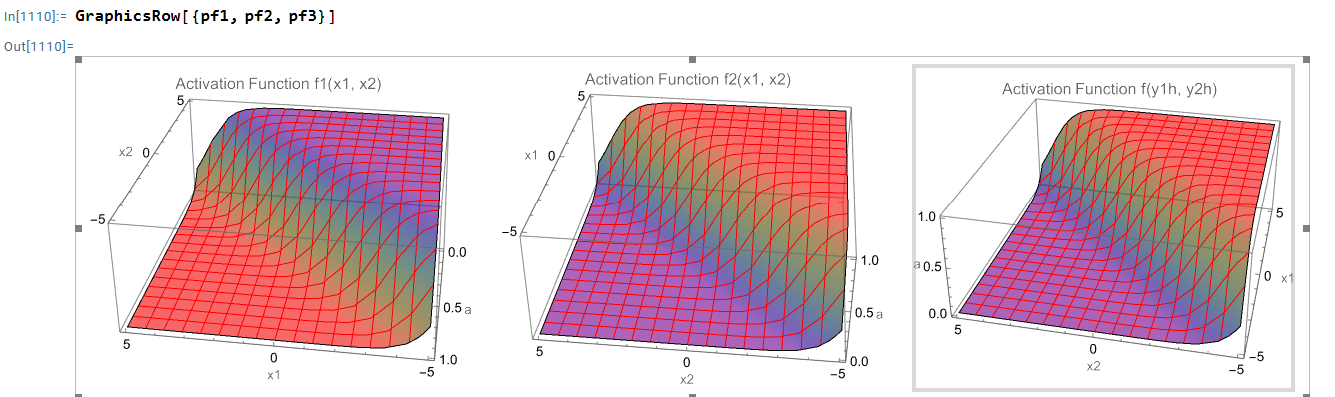
\includegraphics[width=0.8\textwidth]{4_e.PNG}  % Cambia el nombre del archivo y su ruta según sea necesario
  \end{figure}
  \begin{figure}[H]
    \centering
    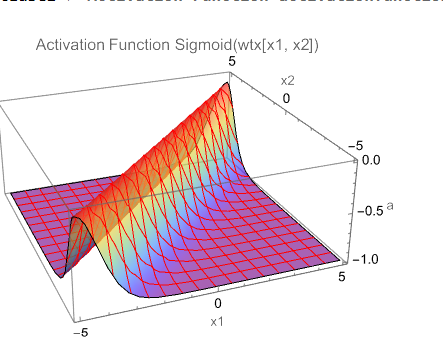
\includegraphics[width=0.5\textwidth]{4_e_2.PNG}  % Cambia el nombre del archivo y su ruta según sea necesario
  \end{figure}

  \item Obtener valores de salida
  
  y1 = 0.731059, 0.952574, 0.731059, 0.268941
  y2 = 0.268941, 0.731059, 0.268941, 0.0474259

  \item Graficar los puntos del ejercicio 6
  \begin{figure}[H]
    \centering
    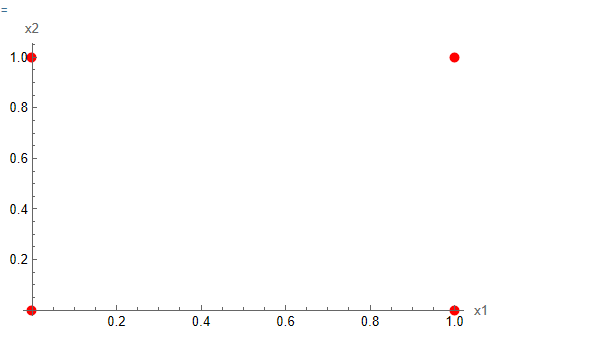
\includegraphics[width=0.5\textwidth]{4_g.PNG}  % Cambia el nombre del archivo y su ruta según sea necesario
  \end{figure}

  \item Graficar los puntos y1h y2h
  \begin{figure}[H]
    \centering
    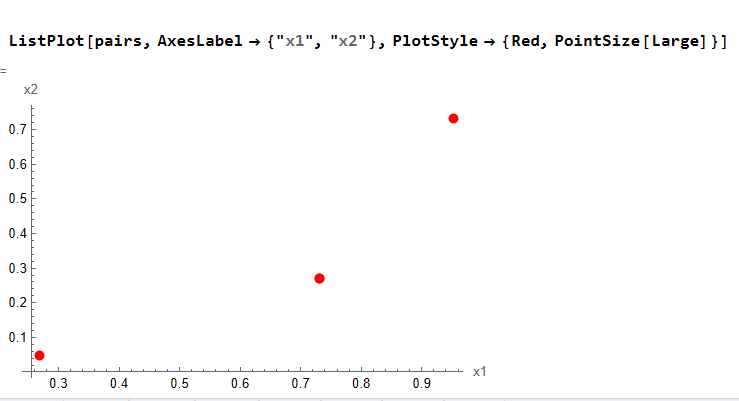
\includegraphics[width=0.5\textwidth]{4_h.PNG}  % Cambia el nombre del archivo y su ruta según sea necesario
  \end{figure}

  \item Verificar que efectivamente (0,0) y (1,1) pertenecen al mismo grupo
  
  0.481068, 0.364249, 0.481068, 0.364249

  \item Encontrar la función de salida para cada neurona (tanh)
\[
\begin{aligned}
  y_1 &= 2\,\tanh\Bigl(2x_1 - 2x_2 + 1\Bigr), \\
  y_2 &= 2\,\tanh\Bigl(-2x_1 + 2x_2 + 1\Bigr), \\
  y_3 &= 2\,\tanh\Bigl(-2x_1 + 2x_2 + 1\Bigr).
\end{aligned}
\]

  \item Obtener la funcion de salida y(x1, x2) con respecto a alas demas entradas x1, x2 de la red neuronal completa$y$.(tanh)
\[
2\,\tanh\Bigl(2x_1 - 2x_2 + 1\Bigr)
+ 2\,\tanh\Bigl(-2x_1 + 2x_2 + 1\Bigr)
- 1
\]
\item Graficar en Geogebra cada una de las funciones obtenidas en los ejercicios 3 y 4 (tanh)
\begin{figure}[H]
  \centering
  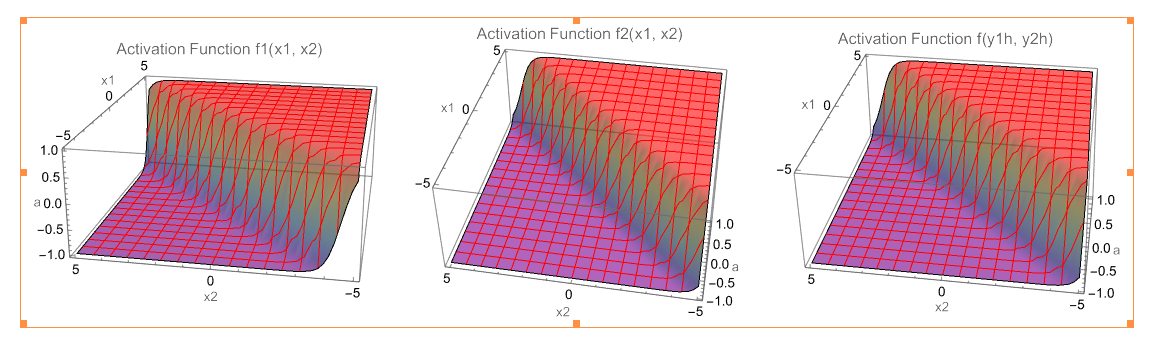
\includegraphics[width=0.8\textwidth]{4_e_tan.PNG}  % Cambia el nombre del archivo y su ruta según sea necesario
\end{figure}
\begin{figure}[H]
  \centering
  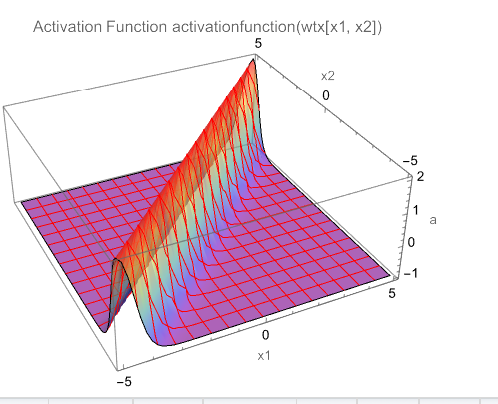
\includegraphics[width=0.8\textwidth]{4_e_tan_final.PNG}  % Cambia el nombre del archivo y su ruta según sea necesario
\end{figure}

\item Obtenga los valores para y1h y y2h (tanh)

\[
y = \begin{pmatrix}
0.761594 & -0.761594 \\
0.995055 & 0.761594 \\
0.761594 & -0.761594 \\
-0.761594 & -0.995055
\end{pmatrix}
\]

\item Graficar y 
\begin{figure}[H]
  \centering
  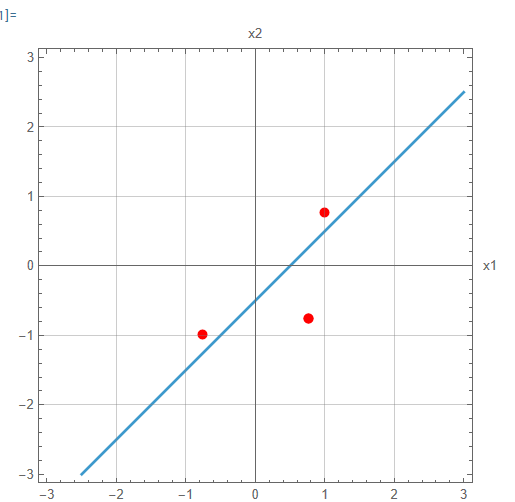
\includegraphics[width=0.8\textwidth]{4_h_tan.PNG}  % Cambia el nombre del archivo y su ruta según sea necesario
\end{figure}

\begin{itemize}
  \item Verifique que efectivamente la red neuronal puede determinar que:
  \begin{enumerate}
    \item $(0,0)$ y $(1,1)$ pertenecen al mismo grupo donde la red neuronal dispara.
    \item $(0,1)$ y $(0,1)$ pertenecen al mismo grupo donde la red neuronal NO dispara.
  \end{enumerate}
\end{itemize}

\[
\begin{array}{cccc}
\colorbox{blue!20}{0.481068} & \colorbox{red!20}{0.364249} & \colorbox{blue!20}{0.481068} & \colorbox{red!20}{0.364249}
\end{array}
\]
  \end{enumerate}
\end{flushleft}
\end{document}